\documentclass[aspectratio=169,11pt]{beamer}

% ── Theme & colors ─────────────────────────────────────────────
\usetheme{metropolis}
\definecolor{DarkNavy}{HTML}{0f172a}
\definecolor{AccentTeal}{HTML}{14b8a6}
\definecolor{AccentPurple}{HTML}{7c3aed}
\definecolor{AccentBlue}{HTML}{60a5fa}
\definecolor{TextLight}{HTML}{f1f5f9}
\definecolor{SoftGray}{HTML}{e2e8f0}
\definecolor{PHBg}{HTML}{f8fafc}
\definecolor{PHBorder}{HTML}{cbd5e1}

\setbeamercolor{normal text}{fg=DarkNavy, bg=white}
\setbeamercolor{frametitle}{bg=DarkNavy, fg=white}
\setbeamercolor{progress bar}{fg=AccentPurple}
\setbeamercolor{alerted text}{fg=AccentPurple}

\usepackage{tikz}
\usetikzlibrary{positioning, arrows.meta, shapes.geometric, calc, backgrounds, fit}
\usepackage{graphicx}
\usepackage{xcolor}
\usepackage{listings}
\usepackage{fontawesome5}

% ── Screenshot placeholder / image helper ──────────────────────
% \screenshot{path}{caption}
% If the file exists it shows the image, otherwise a nice framed placeholder.
\IfFileExists{docs/slides/screenshots/01-docker.png}{}{}
\newcommand{\screenshot}[2]{%
  \begin{center}
  \IfFileExists{#1}{%
    \includegraphics[width=0.82\textwidth,keepaspectratio]{#1}%
  }{%
    \begin{tikzpicture}
      \node[draw=PHBorder, dashed, thick, rounded corners=6pt,
            fill=PHBg, minimum width=0.82\textwidth,
            minimum height=4.2cm, align=center] (box) {};
      \node[align=center, text=DarkNavy] at (box) {%
        \large\textbf{Screenshot placeholder}\\[4pt]
        \small\ttfamily #1\\[6pt]
        \footnotesize\textcolor{gray}{#2}%
      };
    \end{tikzpicture}%
  }%
  \end{center}
}

% ── Command box (shows what to run) ────────────────────────────
\newcommand{\cmd}[1]{%
  \vspace{2pt}
  \begin{center}
  \colorbox{DarkNavy}{%
    \begin{minipage}{0.88\textwidth}
      \vspace{4pt}\color{white}\ttfamily\small \$ #1\vspace{4pt}
    \end{minipage}%
  }
  \end{center}
}

\newcommand{\valueline}[1]{%
  \vspace{4pt}\footnotesize\color{AccentPurple}\faCheckCircle~\textbf{Value:} \color{DarkNavy}#1\par
}

% ── Meta ───────────────────────────────────────────────────────
\title{Regulatory Watch}
\subtitle{Turning regulatory noise into structured compliance signal}
\date{\today}
\author{Regulatory Intelligence Platform}

\begin{document}

% ─────────────────────────────────────────────────────────────
% 1. COVER
% ─────────────────────────────────────────────────────────────
\maketitle

% ─────────────────────────────────────────────────────────────
% 2. VALUE PROPOSITION
% ─────────────────────────────────────────────────────────────
\begin{frame}{The value we deliver}
\vspace{4pt}
\begin{columns}[T,onlytextwidth]
  \column{0.32\textwidth}
    
\begin{tikzpicture}
      \node[draw=AccentPurple, thick, rounded corners=8pt, fill=white,
            minimum width=\linewidth, minimum height=3.2cm, align=center] {%
        \Large\color{AccentPurple}\textbf{95\%}\\[2pt]
        \small\color{DarkNavy}cost saved via\\diff-gated LLM calls
      };
    \end{tikzpicture}
  \column{0.32\textwidth}
    
\begin{tikzpicture}
      \node[draw=AccentTeal, thick, rounded corners=8pt, fill=white,
            minimum width=\linewidth, minimum height=3.2cm, align=center] {%
        \Large\color{AccentTeal}\textbf{100\%}\\[2pt]
        \small\color{DarkNavy}events auditable\\(tokens + \$ logged)
      };
    \end{tikzpicture}
  \column{0.32\textwidth}
    
\begin{tikzpicture}
      \node[draw=AccentBlue, thick, rounded corners=8pt, fill=white,
            minimum width=\linewidth, minimum height=3.2cm, align=center] {%
        \Large\color{AccentBlue}\textbf{138}\\[2pt]
        \small\color{DarkNavy}unit tests\\passing
      };
    \end{tikzpicture}
\end{columns}

\vspace{10pt}
\small
\textbf{From unstructured text to queryable signal:} topic, entities, HS/HTS codes,
origin/destination countries, deadlines, penalties --- all machine-readable.
\end{frame}

% ─────────────────────────────────────────────────────────────
% 3. ARCHITECTURE (one diagram)
% ─────────────────────────────────────────────────────────────
\begin{frame}{Architecture --- one picture, four layers}
\centering
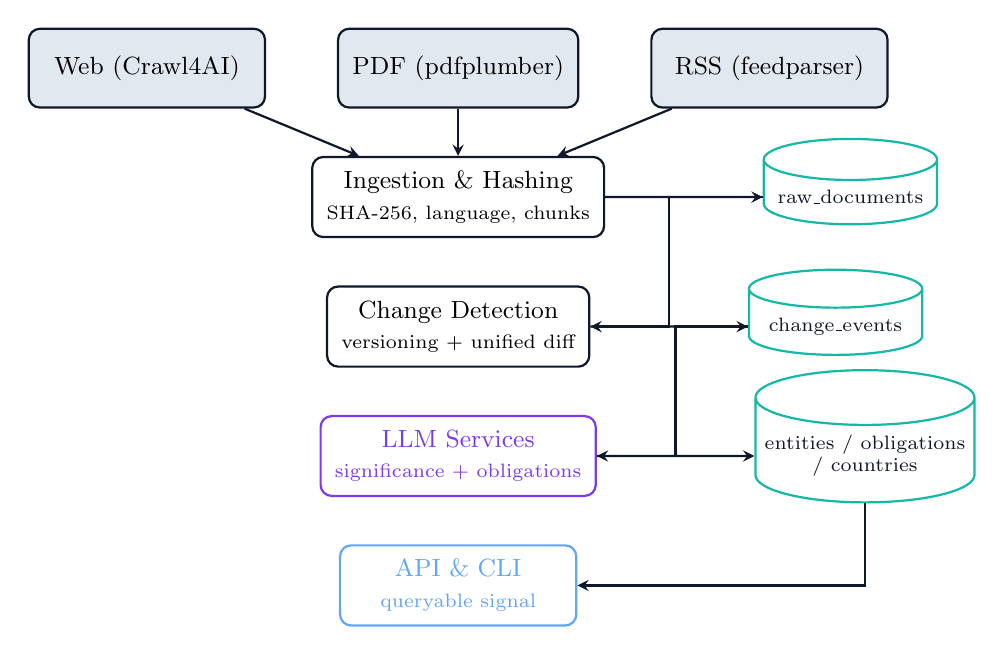
\begin{tikzpicture}[
  node distance=0.6cm and 0.9cm,
  layer/.style={draw=DarkNavy, thick, rounded corners=4pt, fill=white,
                align=center, inner sep=1.2ex, minimum height=1.0cm,
                minimum width=3.0cm, font=\small},
  src/.style={layer, fill=SoftGray},
  llm/.style={layer, draw=AccentPurple, text=AccentPurple},
  db/.style={draw=AccentTeal, thick, cylinder, shape border rotate=90,
             aspect=0.25, fill=white, align=center, minimum height=0.9cm,
             minimum width=2.2cm, font=\scriptsize, text=DarkNavy},
  api/.style={layer, draw=AccentBlue, text=AccentBlue},
  arr/.style={->, >=stealth, thick, DarkNavy}
]
  % Layer 1: sources
  \node[src] (web)  {Web (Crawl4AI)};
  \node[src, right=of web] (pdf)  {PDF (pdfplumber)};
  \node[src, right=of pdf] (rss)  {RSS (feedparser)};

  % Layer 2: ingestion
  \node[layer, below=of pdf] (ingest) {Ingestion \& Hashing\\\scriptsize SHA-256, language, chunks};
  \node[db, right=2.0cm of ingest] (raw) {raw\_documents};

  % Layer 3: change detection
  \node[layer, below=of ingest] (diff) {Change Detection\\\scriptsize versioning + unified diff};
  \node[db, right=2.0cm of diff] (ev) {change\_events};

  % Layer 4: LLM
  \node[llm, below=of diff] (llm) {LLM Services\\\scriptsize significance + obligations};
  \node[db, right=2.0cm of llm] (out) {entities / obligations\\/ countries};

  % Output
  \node[api, below=of llm] (api) {API \& CLI\\\scriptsize queryable signal};

  % Arrows sources -> ingest
  \draw[arr] (web)  -- (ingest);
  \draw[arr] (pdf)  -- (ingest);
  \draw[arr] (rss)  -- (ingest);

  \draw[arr] (ingest) -- (raw);
  \draw[arr] (raw)    -| ($(diff.east)+(1.0,0)$) -- (diff.east);
  \draw[arr] (diff)   -- (ev);
  \draw[arr] (ev)     -| ($(llm.east)+(1.0,0)$) -- (llm.east);
  \draw[arr] (llm)    -- (out);
  \draw[arr] (out)    |- (api);
\end{tikzpicture}
\end{frame}

% ─────────────────────────────────────────────────────────────
% 5. DEMO 1 — STACK UP
% ─────────────────────────────────────────────────────────────
\begin{frame}{Demo 1 --- Stack up}
\cmd{docker compose up -d}
\screenshot{docs/slides/screenshots/01-docker.png}{Expected: API, worker, Postgres, Redis running.}
\valueline{One command brings up the full production-grade stack (5 services).}
\end{frame}

% ─────────────────────────────────────────────────────────────
% 6. DEMO 2 — INGESTION
% ─────────────────────────────────────────────────────────────
\begin{frame}{Demo 2 --- Ingestion run}
\cmd{docker compose exec worker python scripts/ingest\_urls.py --limit 5}
\screenshot{docs/slides/screenshots/02-ingest.png}{Expected: 5 raw\_documents stored, SHA-256 logged per URL.}
\valueline{Heterogeneous sources (HTML + PDF + RSS) unified into one clean pipeline.}
\end{frame}

% ─────────────────────────────────────────────────────────────
% 7. DEMO 3 — CHANGE DETECTION
% ─────────────────────────────────────────────────────────────
\begin{frame}{Demo 3 --- Change detection}
\cmd{docker compose exec worker python scripts/show\_changes.py}
\screenshot{docs/slides/screenshots/03-changes.png}{Expected: list of change\_events with diff\_kind + char deltas.}
\valueline{Only \emph{real} changes reach the LLM --- massive cost reduction on stable pages.}
\end{frame}

% ─────────────────────────────────────────────────────────────
% 8. DEMO 4 — SIGNIFICANCE + TOPIC
% ─────────────────────────────────────────────────────────────
\begin{frame}{Demo 4 --- Significance \& topic}
\cmd{docker compose exec worker python scripts/show\_changes.py --scored}
\screenshot{docs/slides/screenshots/04-significance.png}{Expected: score, change\_type, topic, origin countries, summary.}
\valueline{Raw text $\rightarrow$ scored, classified, summarized in a single LLM call.}
\end{frame}

% ─────────────────────────────────────────────────────────────
% 9. DEMO 5 — OBLIGATIONS
% ─────────────────────────────────────────────────────────────
\begin{frame}{Demo 5 --- Structured obligations}
\cmd{docker compose exec worker python scripts/show\_obligations.py}
\screenshot{docs/slides/screenshots/05-obligations.png}{Expected: actor / action / deadline / penalty rows.}
\valueline{Unstructured prose $\rightarrow$ machine-readable duties. Ready for dashboards \& alerts.}
\end{frame}

% ─────────────────────────────────────────────────────────────
% 10. DEMO 6 — ENTITIES & COUNTRIES
% ─────────────────────────────────────────────────────────────
\begin{frame}{Demo 6 --- Entities, HS codes \& countries}
\cmd{docker compose exec worker python scripts/show\_entities.py}
\screenshot{docs/slides/screenshots/06-entities.png}{Expected: HS/HTS codes (0304.29.00…), agencies, regulations, ISO-2 countries.}
\valueline{Every event is queryable by country, agency, regulation, and tariff code.}
\end{frame}

% ─────────────────────────────────────────────────────────────
% 11. DEMO 7 — COST REPORT
% ─────────────────────────────────────────────────────────────
\begin{frame}{Demo 7 --- LLM cost \& token report}
\cmd{docker compose exec worker python scripts/llm\_cost\_report.py}
\screenshot{docs/slides/screenshots/07-cost.png}{Expected: tokens in/out + USD total per scope (significance / obligations).}
\valueline{Every LLM call is logged --- full financial \& audit transparency.}
\end{frame}

% ─────────────────────────────────────────────────────────────
% 12. QUALITY PROOF
% ─────────────────────────────────────────────────────────────
\begin{frame}{Quality \& resilience proof}
\begin{itemize}
  \item \textbf{138 unit tests} covering ingestion, diff, entity index, geo, schema.
  \item \textbf{Alembic migrations} --- no stray \texttt{create\_all} in production.
  \item \textbf{Circuit breaker} (Redis-backed) protects against OpenAI outages.
  \item \textbf{Structured logs + LLM ledger} --- every call traceable to \$.
  \item \textbf{Rate limits} on Celery tasks --- no runaway cost.
\end{itemize}
\screenshot{docs/slides/screenshots/08-tests.png}{Expected: pytest output --- 138 passed.}
\end{frame}

% ─────────────────────────────────────────────────────────────
% 13. WHAT'S NEXT
% ─────────────────────────────────────────────────────────────
\begin{frame}{What's next}
\begin{itemize}
  \item \textbf{Alert delivery:} email / Slack / webhooks on saved queries.
  \item \textbf{Dashboard UI:} visualize events, entities, obligations.
  \item \textbf{More connectors:} Federal Register API, EUR-Lex API, WTO feeds.
  \item \textbf{Human-in-the-loop:} review queue to correct LLM extractions.
  \item \textbf{Embeddings \& semantic search:} topical clustering across agencies.
\end{itemize}
\end{frame}

% ─────────────────────────────────────────────────────────────
% 14. THANKS
% ─────────────────────────────────────────────────────────────
\begin{frame}[standout]
  Thank you\\[6pt]
  \normalsize Questions?
\end{frame}

\end{document}
